\documentclass{bmvc2k}

%% Enter your paper number here for the review copy
%\bmvcreviewcopy{??}

%\title{Bringing Real Objects into the Digital World Through Observation}
\title{See, Spawn, Synchronize: A Digital Twin Pipeline for Smart Production Cells}

% Enter the paper's authors in order
% \addauthor{Name}{email/homepage}{INSTITUTION_CODE}
\addauthor{Malte Herrmann}{malte.herrmann@ovgu.de}{1}
\addauthor{Ayoub Al-Hamadi}{}{1}

% Enter the institutions
% \addinstitution{Name\\Address}
% \addinstitution{
%     Neuro-Information Technology Group,\\
%     Otto-von-Guericke-University, \\
%     Magdeburg, Germany
% }

\addinstitution{
Otto von Guericke University Magdeburg,\\
Neuro-Information Technology Group,\\
Universitätsplatz 2,\\
39106 Magdeburg
}

%\runninghead{Herrmann, Al-Hamadi}{From Observation to Digital Objects}
\runninghead{Herrmann, Al-Hamadi}{Digital Twins for Smart Production Cells}

% Any macro definitions you would like to include
% These are not defined in the style file, because they don't begin
% with \bmva, so they might conflict with the user's own macros.
% The \bmvaOneDot macro adds a full stop unless there is one in the
% text already.
\def\eg{\emph{e.g}\bmvaOneDot}
\def\Eg{\emph{E.g}\bmvaOneDot}
\def\etal{\emph{et al}\bmvaOneDot}

%-------------------------------------------------------------------------
% Document starts here
\begin{document}

\maketitle

\begin{abstract}
With Industry 5.0, human-robot collaboration has moved to the center of attention. This opens a problem, where workspaces become highly dynamic leading to safety concerns for robots and especially for humans. This makes it important to have a realistic and precise image of a production cell and its components in the environments for movement planning and damage prevention.

This paper presents a digital twin of an Industry 5.0 smart production cell, that synchronizes objects in the real-world workspace with minimal effort, requiring only an RGB-D camera. A fine-tuned version of the YOLO network detects cubes in the scene and estimates their position and top-side letter. After coordinate transformation, these objects are spawned in \textit{Unity} at the exact location relative to the robot. This process has been successfully demonstrated in experiments where the use of fiducial markers enables precise placement. Once the cubes have been spawned, they can be moved via drag-and-drop within the simulation. Once such changes have been confirmed, a movement planning node calculates a trajectory to carry out the displacement and synchronize both production cells.


% This document demonstrates the format requirements for papers submitted
% to the British Machine Vision Conference.  The format is designed for
% easy on-screen reading, and to print well at one or two pages per sheet.
% Additional features include: pop-up annotations for
% citations~\cite{Authors06,Mermin89}; a margin ruler for reviewing; and a
% greatly simplified way of entering multiple authors and institutions.

% {\bf All authors are encouraged to read this document}, even if you have
% written many papers before.  As well as a description of the format, the
% document contains many instructions relating to formatting problems and
% errors that are common even in the work of authors who {\em have}
% written many papers before.

\end{abstract}

%-------------------------------------------------------------------------
\section{Introduction}
\label{sec:intro}
Digital relatives, such as digital twins (DT)~\cite{singh_digital_2021} and digital cousins (DC)~\cite{dai2024automated}, have become more popular in recent years. This is mostly due to their ability to quickly adapt to changing environments, prevent damage and consume less energy than industrial robots~\cite{landscheidt_method_2016}. Another advantage is that the movement of the real robot can be planned remotely in advance. This allows helps avoid possible collisions with other robots or the environment. This works quite well in cases of static surroundings, but when it comes to dynamic changes, such as the position and orientation of tools or products, the digital space needs to adapt. This paper presents an environment for a production cell that creates a representation of the current workspace by scanning it with an RGB-D camera only. AI nodes generate clones that can be moved and manipulated. These changes are then fed back to the real robot control system, which performs the planned movement. This technology is ideal for important Industry 5.0 applications, and its functionality is based on the digital twin environment described in ~\cite{herrmann2025realtime}.

In addition to remotely controlling the DT, this functionality allows real-world circumstances and tasks to be set up and transferred into the digital realm. There, reinforcement learning can be applied to the simulation. This reduces the gap between simulation and reality.


The accuracy of the placement of the creates objects is validated in an experiment. XX


\section{Related Works}
\label{sec:SOTA}
A lot of different digital twins with different purposes have been developed. In \cite{xiang_development_2024}, the DT is used as a tool to visualize and control an entire work task. A comparison between controlling a real and a digital robot by teaching and a Virtual Reality (VR) user interface leads to a similar task efficiency~\cite{kuts_digital_2022}. To enlarge the usability, a DT framework with haptic feedback has been developed in~\cite{fan_digital_2023}. Air-filled pockets indicate to the user whether the gripper has grabbed an object and how stiff the material is. Another approach to control a physical robot via its digital representative has been made in~\cite{chang_construction_2025}. A graphical user interface (GUI) has been deployed as a control platform, which simplifies the programming of industrial robots. In~\cite{kawshan_digital_2026} a framework has been developed, that can be used for path planning and real-time execution of robot arms.
All mentioned approaches above are using the game engine \textit{Unity} as the development platform, and some connect to the robot networks via ROS/ROS2.

When it comes to reproducing the real workspace, some DTs use Mixed Reality (MR), in which objects are projected into the user's view. This is achieved by either detecting fiducial markers or object detection. The system then creates objects that are visible to the user. In \cite{gallala_digital_2022} the first method is used to overlay the digital representative directly on the real robot to show the calculated trajectory.


The object detection method is used in \cite{wu_teleoperation_2025}. A MR framework displays colored cubes, which are detected by an object detector utilizing the RGB-D Image date of the workspace, in a virtual scene. With a VR Headset and Controller, the cubes can be moved to indirect teleoperate the robot arm.


Various approaches have been made to digitalize the surroundings of a robot and manipulating.




XX
\newpage
\section{Method}
\label{sec:method}
To achieve valuable results, the digital production cell should be recreated as accurately as possible. A precise rebuild helps to reduce the gap between simulation and reality. Figure \ref{fig:production_cell} compares both types of production cell
\begin{figure}[h]
    \centering
    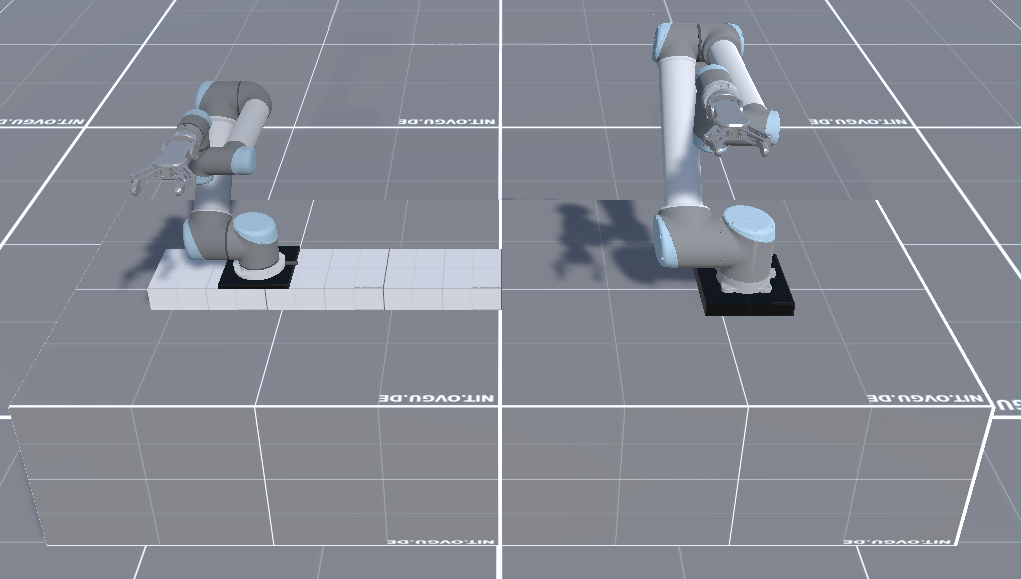
\includegraphics[width=0.49\linewidth]{media/Production_cell.png} %left
    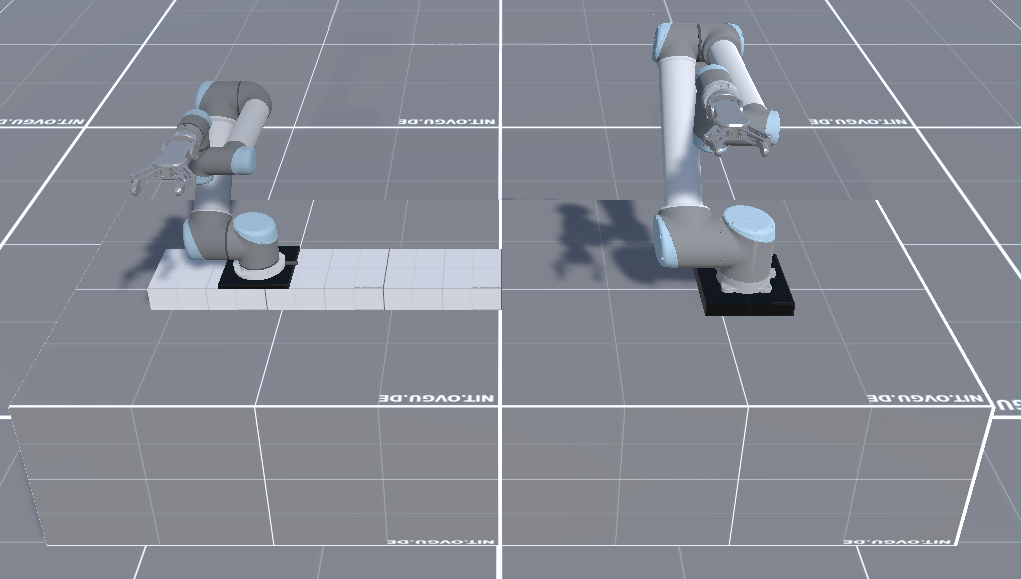
\includegraphics[width=0.49\linewidth]{media/Production_cell.png} %right
    \caption{Both production cells. \textit{left}: real world, \textit{right}: digital world.}
    \label{fig:production_cell}
\end{figure}

There are three different operating modes of the digital twin. First, it can act as a digital shadow that only displays the current robot configuration and AI node states. This supports user to supervise the current Robot state, even when being remotely far away. Secondly, the DT operates as a movement planning tool. When objects are moved, commands are sent to the real robot system to recreate these changes. This planning can also be carried out remotely. Finally, the DT can be used for simulation and reinforcement learning purposes without real hardware. 

The whole system, including real robot and DT can be divided in four parts, which are explained in this section. As shown in Figure~\ref{fig:schematic}, collected data from the real-world robots (~\ref{rw:robots}) is interpreted by AI nodes (~\ref{dw:perception}). This information is then interpreted by the Digital Twin software (~\ref{dw:DT}) and implemented in the environment. After modifications, algorithms are used to apply the changes to the real-world environment (~\ref{dw:algo}).

\begin{figure}[h]
    \centering
    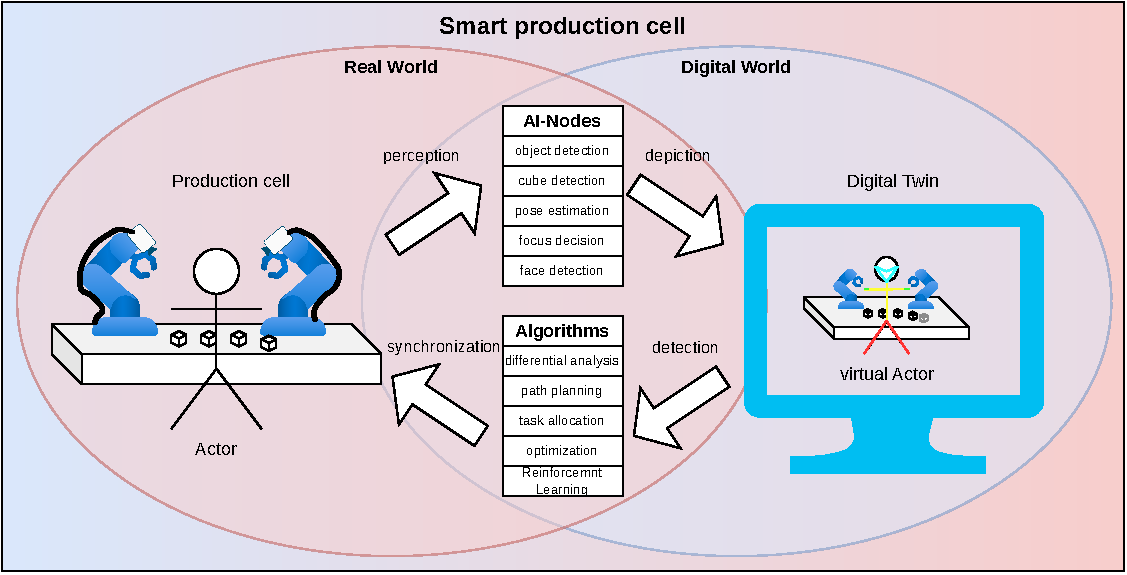
\includegraphics[width=\linewidth]{media/scematic_production_cell_neu.pdf}
    \caption{The schematic diagram of the smart production cell. Real-world camera data is perceived and interpreted by AI nodes. Then, the information is prepared and depicted to be included in the digital twin. Any changes made there are detected and processed to synchronize the real workspace.}
    \label{fig:schematic}
\end{figure}

\subsection{Real-world setup}
\label{rwsetup}
The real-world setup describes the hardware modalities as well as the objects contained in the workspace.

\subsubsection{Robots}
\label{rw:robots}
The real smart production cell consists of two kinematic chain robots from \textit{Universal Robots} located in a line on the table. The smaller UR5e robot on the left is mounted on a linear axis that is not in use. It has an RG6 gripper by \textit{OnRobot} installed at the tool flange. On the right-hand side of the table is an UR10e robot. This robot is equipped with a 2FR14 gripper also by \textit{OnRobot}. Both robots are using \textit{Intel} \textit{RealSense} D435 RGB-D cameras mounted on top of their grippers.

Both robots run an individually adapted version of the original Universal Robots driver software to ensure execution on a single PC without topics with the same name being mixed. These namespaces are essential for distinguishing the robots in the simulation and enabling inter-robot communication.

\subsubsection{Workspace}
\label{rw:workspace}
The robots' work area covers the entire table. The left, respective the right-hand side belongs only to the dedicated robot. In the middle a shared workspace is defined, enabling object passing.
physical markings can be placed in the holes of the table to indicate defined positions. Due to their defined size, these markings can also be transferred to the simulation for validation purposes.

As objects, black and white cubes are used. The 3D-printed cubes have a length of $5\,\mathrm{cm}$ in each dimension and a different letter on each side. This helps to distinguish the recognized cubes in the simulation. 

\subsection{Digital-world setup}
\label{dw:setup}
In the digital world, all the components of the functional digital twin come together. Cameras mounted on the real robot gather images, which are interpreted by AI nodes. This information is then used to recreate the workspace in the simulation. The simulation is implemented in \textit{Unity} and connected to the ROS2 domain via a TCP endpoint. \textit{Unity}, as a gaming engine, offers the possibility to manipulate and interact with objects in multiple ways. Currently, interaction is only possible via the PC mouse. Later, integrating Virtual Reality or interacting with the pose estimation model will be possible with ease. Once the user has acknowledged the changes, the state is sent via ROS2 to the path planning nodes, which send commands to the real robot controller to accomplish the task. More detail is provided in the following subsections.

\subsubsection{AI-Perception}
\label{dw:perception}
XX: kann auf roboter system oder DT PC laufen
The RGB and depth images transferred via the ROS2 network are fed into multiple AI nodes. For object/cube detection, a simple YOLO[XX] network is used that has been finetuned with data from the black and white cubes used for the task. The output provides information about the position and orientation in the image, and the type of object, respectively, the topside letter. To determine the distance to the camera, the depth image is taken into account. The depth value is piked at the intersection point of the diagonals of the bounding boxes.

XXHelpernode
For the cube spawning, a ROS2 helper node was developed. It subscribes to the bounding boxes topic and translates this information to be interpretable by Unity. The cube spawn point is calculated with respect of the camera position with help of the intrinsic camera parameter. Because \textit{Untiy} implicit has transformation matrices for the kinematic joints of the robot, the extrinsic camera parameter are only used for the placement of the camera. Because the depth images only provide the distance to the topside and the origin of the cube is in the middle, a small offset of $2.5\,\mathrm{cm}$ need to be taken into account.

%XX Das hier brauche ich gar nicht, da das tracking nicht mit rein kommt
%The pose estimation node uses mmpose [XXgenaues Modell erwähnen\url{https://mmpose.readthedocs.io/en/latest/model\_zoo\_papers/algorithms.html}]  to estimate the skeletal posture (COCO 17-Point Keypoint Names [XX]) of people standing in front of the camera. The distance of each point is, as well, taken from the depth image. This makes it possible to display the person's model correctly in front of the robot.

%Beside the perception nodes, decision nodes are determine, what object or which person gets the focus of the robot. XXIn real production cells this is relevant to communicate to the worker[IMHERE-PaperXX].   detectThose nodes function as object or face detection and pose estimation. This information, consisting of skeletal posture and oriented bounding boxes, is then interpreted by the Digital Twin software and implemented in the environment. The user can then manipulate objects inside the simulation. After the planned movement has been acknowledged, algorithms detect changes in the environment and start trajectory planning, which is then applied to the real and digital robots performing the action simultaneously.
\subsubsection{Digital Twin}
\label{dw:DT}
\textit{Unity} was chosen for the implementation of the digital twin, because of the variety of opportunities. The dynamic and presentable visualization of models and objects, in combination with an included physics engine makes it the optimal tool~\cite{singh_unity_2024}. The table has been rebuild by scale. 1 unit in \textit{Unity} corresponds to $1\,\mathrm{m}$ in the real world. The robot and gripper models have been imported with the help of an URDF-Importer~\footnote{\url{https://github.com/Unity-Technologies/URDF-Importer}}, provided by \textit{Unity} itself. With the TCP endpoint, the joint states topic from the real robot is subscribed and applied to the models joints. This mirrors the actual movement in real-time.

A helper ROS2 node is used to create the objects. This node subscribes to the estimated bounding boxes of cube detection, transforms the received pixel coordinates into world coordinates, and sends a command to \textit{Unity} to spawn a distinct cube at the calculated position. The node also keeps track of cubes that have already been detected to prevent the same cube being spawned multiple times.

The spawn root point is defined at the position of the robot model where the camera is typically located. Due to the underlying URDF files, the positioning can be made very precise. Since the AI nodes output data relative to the camera frame, no further calculations are required except for translating pixel coordinates to world coordinates.

Once spawned, the cubes can be moved around the workspace using the PC mouse. They can be placed on the table or stacked on top of each other. To help with visualization, a ghost version of the cube appears in the simulation to indicate the target position. (see Fig~\ref{XX}).

The user interface provides an acknowledgement button for the changes. Clicking the button sends a ROS2 message to the execution planning node, which is described in subsection~\ref{subsec:execution}. As the simulation is still subscribed to the joint states topic, both the execution of the real robot task and the movement of the virtual cube are displayed, taking into account the physics engine.


\subsubsection{Task execution planning}
\label{dw:algo}
\label{subsec:execution}
Task execution planning is also a helper node. The message sent from \textit{Unity} contains the cube's current position and the designated new position in the workspace. When stacking cubes, the motions are sorted by z-value to ensure that the cubes are not placed in mid-air, while stacking them.
To ensure safe movement, the table's dimensions are sent to \textit{moveIt}~\footnote{\url{https://moveit.ai/}}, a motion planning framework. Using this information, it can calculate possible paths. The complete task is divided into eight sub-tasks. These cover the approach to the cube, grasping it, and the actual movement. The helper sends these movement points to the running \textit{moveIt} node, where a trajectory is calculated. Since the gripper is included in the URDF and SRDF files, its trajectory is also calculated via \textit{moveIt}, which sends commands to a separate gripper controller. This process is repeated for every displaced cube in the simulation.


\section{Experiment}
\label{sec:experiment}

Two experiments were conducted during development. The first demonstrates the accuracy with which the cubes are detected and placed in the simulation workspace. Based on this, the cubes are moved, and the path planning algorithm aligns the placement in the second experiment.

\subsection{Cube placement / Workspace scanXX}
\label{ex:placement}
This experiment validates the precision of the cube detection for recreating the current workspace, making it possible to transition cube positions in a remote environment.

\subsubsection{Setup}
The real table represents the workspace and has holes drilled at $2.5\,\mathrm{cm}$ intervals. These holes are used to determine placement. Due to the visual difference between the real table and the one in the simulation, the positions of the holes were measured from the edges of the table. The position of the right front hole is indicated in red/blue/pink. All fiducial marker have been positioned according to the original from this origin.

These 3D-printed markers simplify cube positioning in the real world. This is because a slope enables the cubes to slide into position. They fit exactly in the holes of the table. In the simulation, they function as a fiducial marker and are placed in specific locations.
Two types of marker have been designed. One type keeps the cube on the table surface and the other lifts it to a height of $5\,\mathrm{cm}$. Both types are shown in Fig.~\ref{fig:cubeholder}.
Some markers are left empty as placeholders for the second experiment.
XX Das hier kann vielleicht noch ausgeschmückt werden.

%XXIn the simulation, the texture of the table has been edited to have markings on the surface, that correspond to the holes in the table. They have a distance of $2.5\,\mathrm{cm}$ on the XZ-plane. Two 3D-printed templates, each with an edge length of approx. $5\,\mathrm{cm}$, are used to fixate the cubes. They are shown in Fig.~\ref{fig:cubeholder}. These templates define the cubes to the surface, and at a height of $5\,\mathrm{cm}$. These templates fit in the holes of the table and are also located in the digital twin environment.

%The table represents the workspace and has holes drilled at 2.5 cm intervals. These holes are used to determine placement. In the simulation, the texture of the table has been edited to include markings on its surface that correspond to the holes. These markings are spaced 2.5 cm apart on the XZ plane. Two 3D-printed templates, each with an edge length of approximately 5 cm, are used to fix the cubes in place. They are shown in Fig.~\ref{fig:cubeholder}. These templates fix the cubes to the surface at a height of 5 cm. The templates fit into the holes in the table and are also located in the digital twin environment.

\begin{figure}[h]
    \centering
    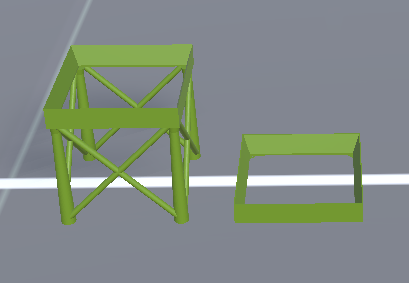
\includegraphics[width=0.49\linewidth]{media/cube_templates.png}
    %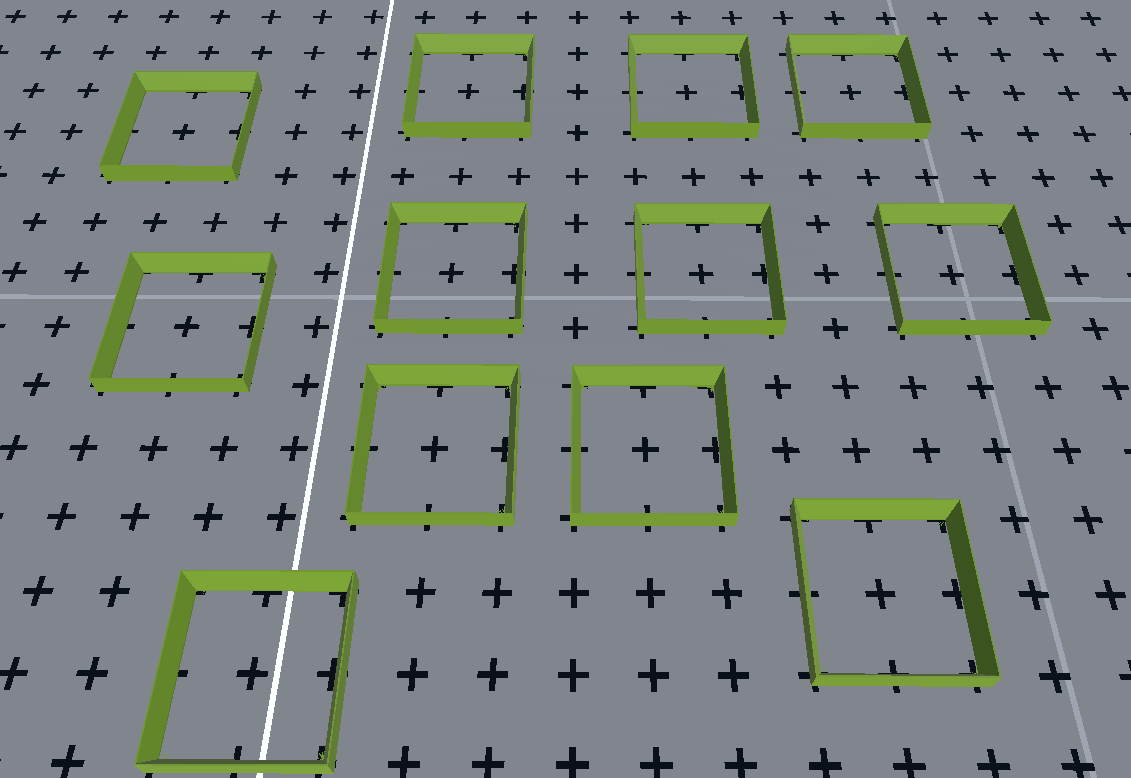
\includegraphics[width=0.49\linewidth]{media/GridWithTemplates.png}
    \caption{The rebuild workspace. left: models of the fiducial marker, right: positioning of the markers in the workspace.XX hier oder unten}
    \label{fig:cubeholder}
\end{figure}

For the experiment, cubes are now placed inside these markers in the real world. The color and the top side letter is determined by random. To ensure this, the cubes are poured out of a box and then sorted to the next template. This procedure can be seen in Video XX.

XX Bild vom Workspace
\begin{figure}[h]
    \centering
    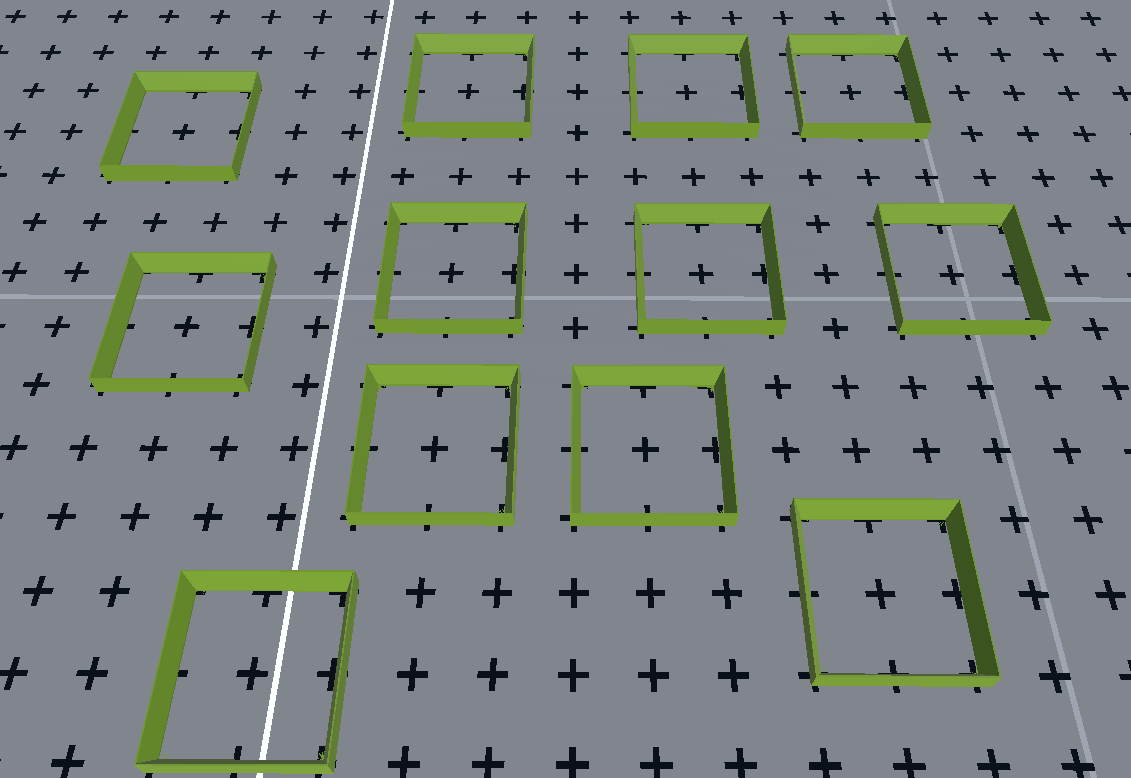
\includegraphics[width=0.49\linewidth]{media/GridWithTemplates.png}
    \caption{Both workspaces before the experiment. \textit{left}: real, \textit{right}: simulation.}
    \label{fig:cubeholder}
\end{figure}

\subsubsection{Procedure}
In order to reproduce the current real workspace, it is scanned using the RGB-D camera mounted on the robot. A trajectory is planned to move the tool center point orthogonally to the table's surface. Starting at the right-most side, it moves at a constant speed parallel to the long edge to the left-most side. During this movement, the cube detection node estimates the pixel coordinates of the bounding box. Using this information, the cube spawner node calculates the world coordinates by using the intrinsic camera parameters and depth values. This pose information is then sent to and interpreted by \textit{Unity}, where the cubes are spawned with the detected top-side letter. 

\subsubsection{Evaluation}

\subsection{Cube movement}
The second experiment demonstrates that it is possible to plan a movement in the digital twin that is then executed in the real world.

\subsubsection{Setup}
The scanned workspace from the previous experiment is used as a basis. The start position of the robot is the predefined home position. As a placement option the additionally placed empty markers can be used. A placement in between is also possible.


Cubes can now be moved around the workspace at will and placed anywhere inside it, even on the marker. This is achieved by using the drag-and-drop function with the PC mouse. A ghost model is displayed to indicate the cube's new position. Once the task is complete, this ghost model can be used to validate the placement.


\subsubsection{Procedure}
In \textit{Unity}, an arbitrary number of cubes are selected and moved in the XZ plane. To demonstrate the precision of the placement, a pyramid consisting of four stacked cubes is created. Once the displacement is complete, the changes are acknowledged by pressing the 'Move Cube' button in the GUI. This starts the trajectory calculation by sending the source and target poses to the movement planning node. Since this node only prepares positions that can be interpreted by MoveIt, it is not taken into consideration any further.

\subsubsection{Evaluation}

\begin{figure}[h]
    \centering
    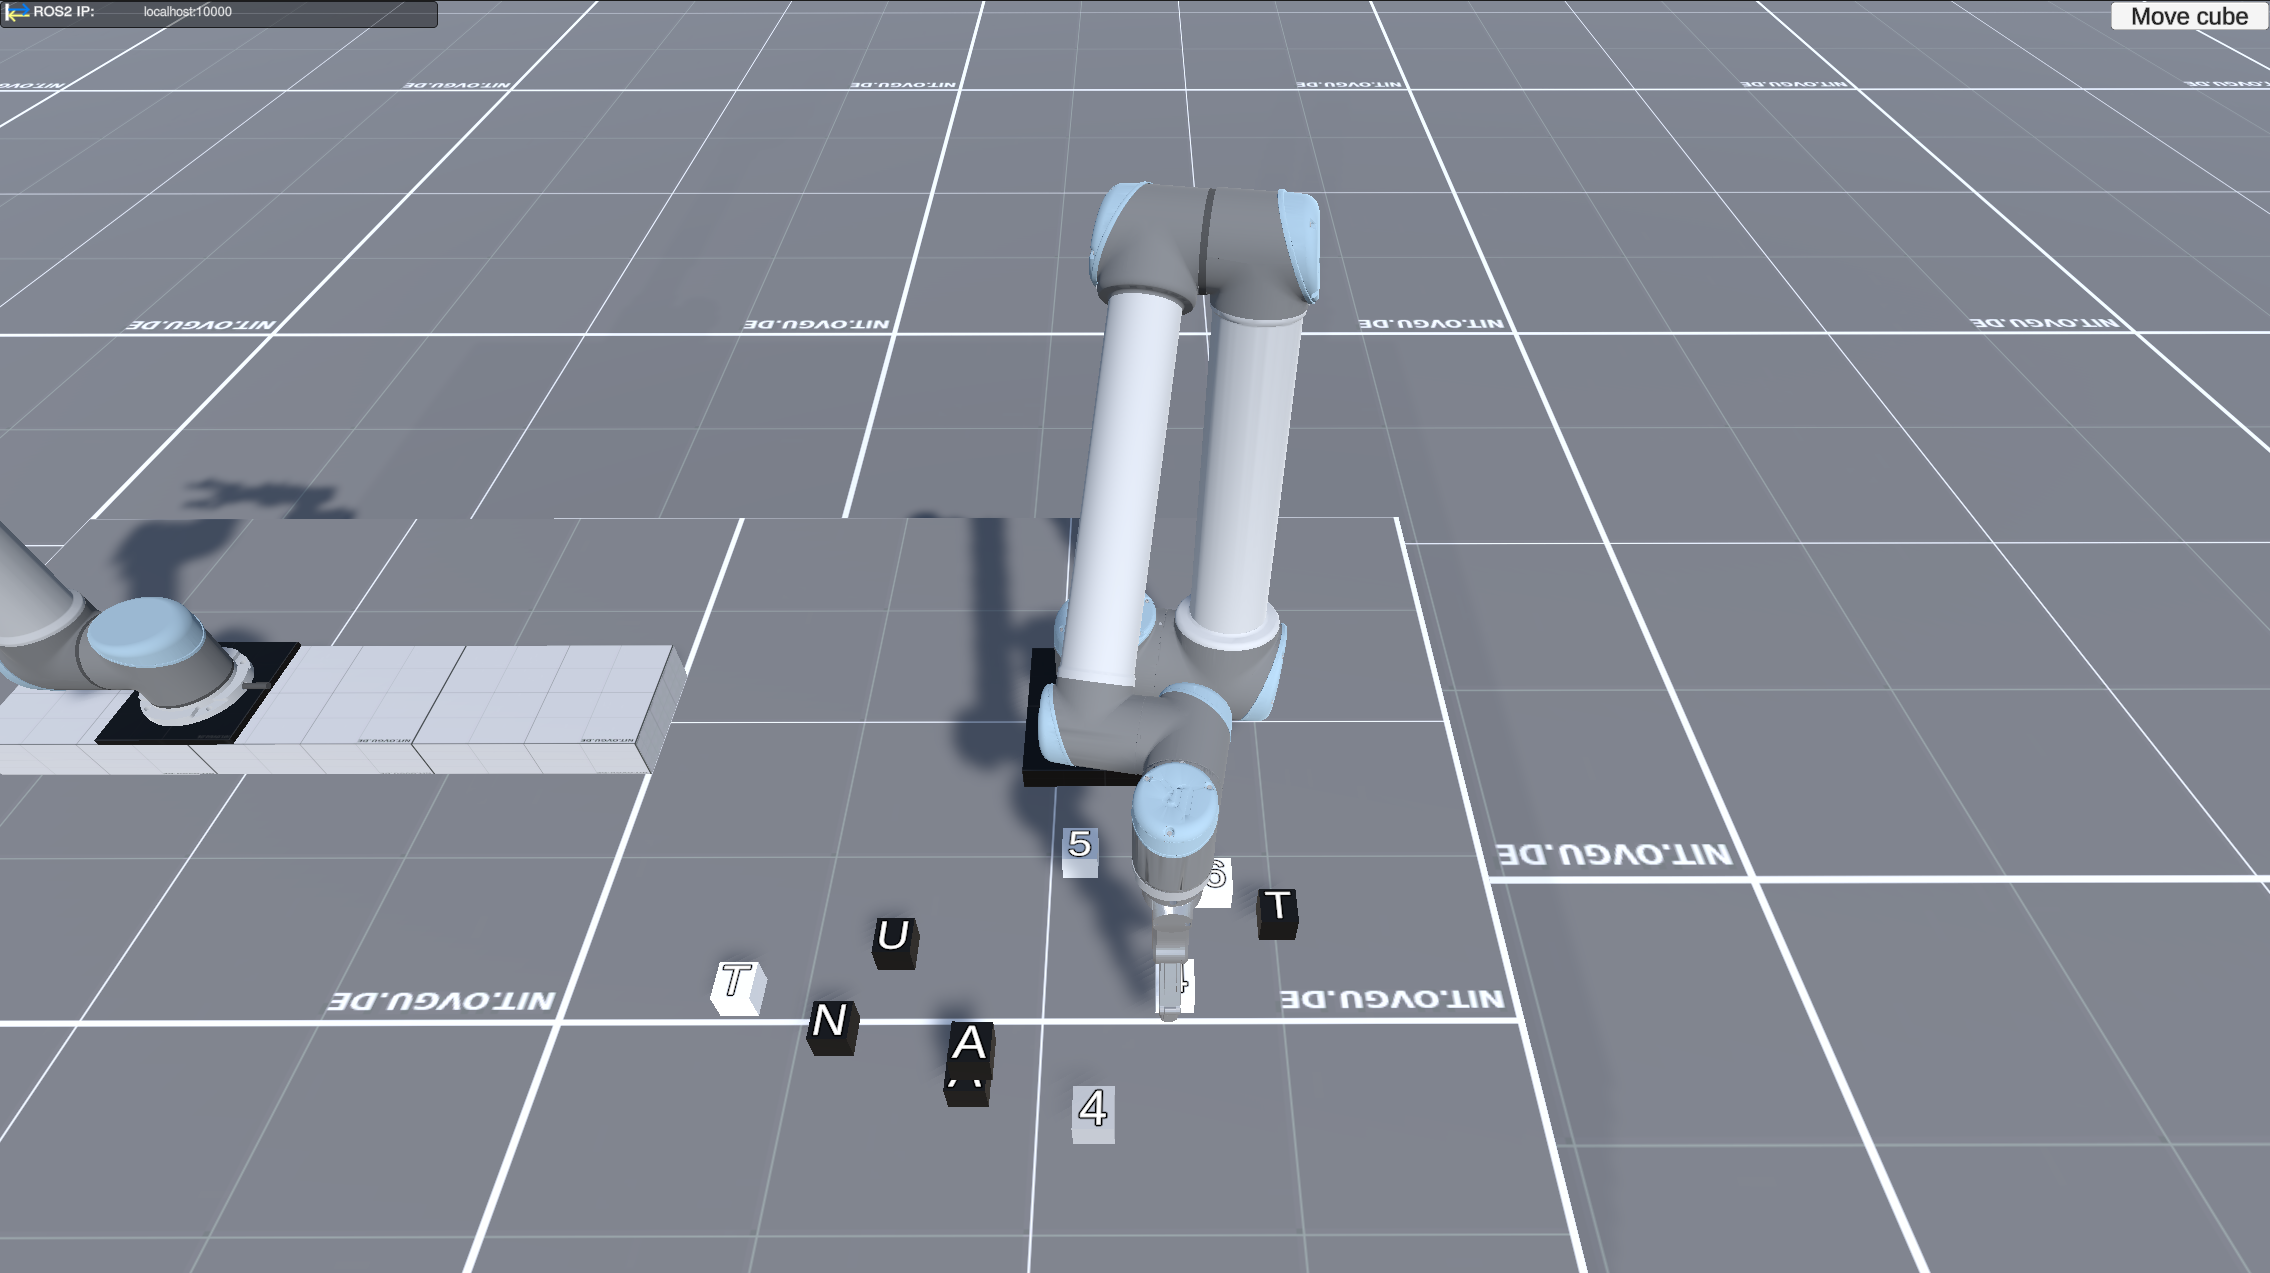
\includegraphics[width=0.3\linewidth]{media/Workspace 1_017.png}
    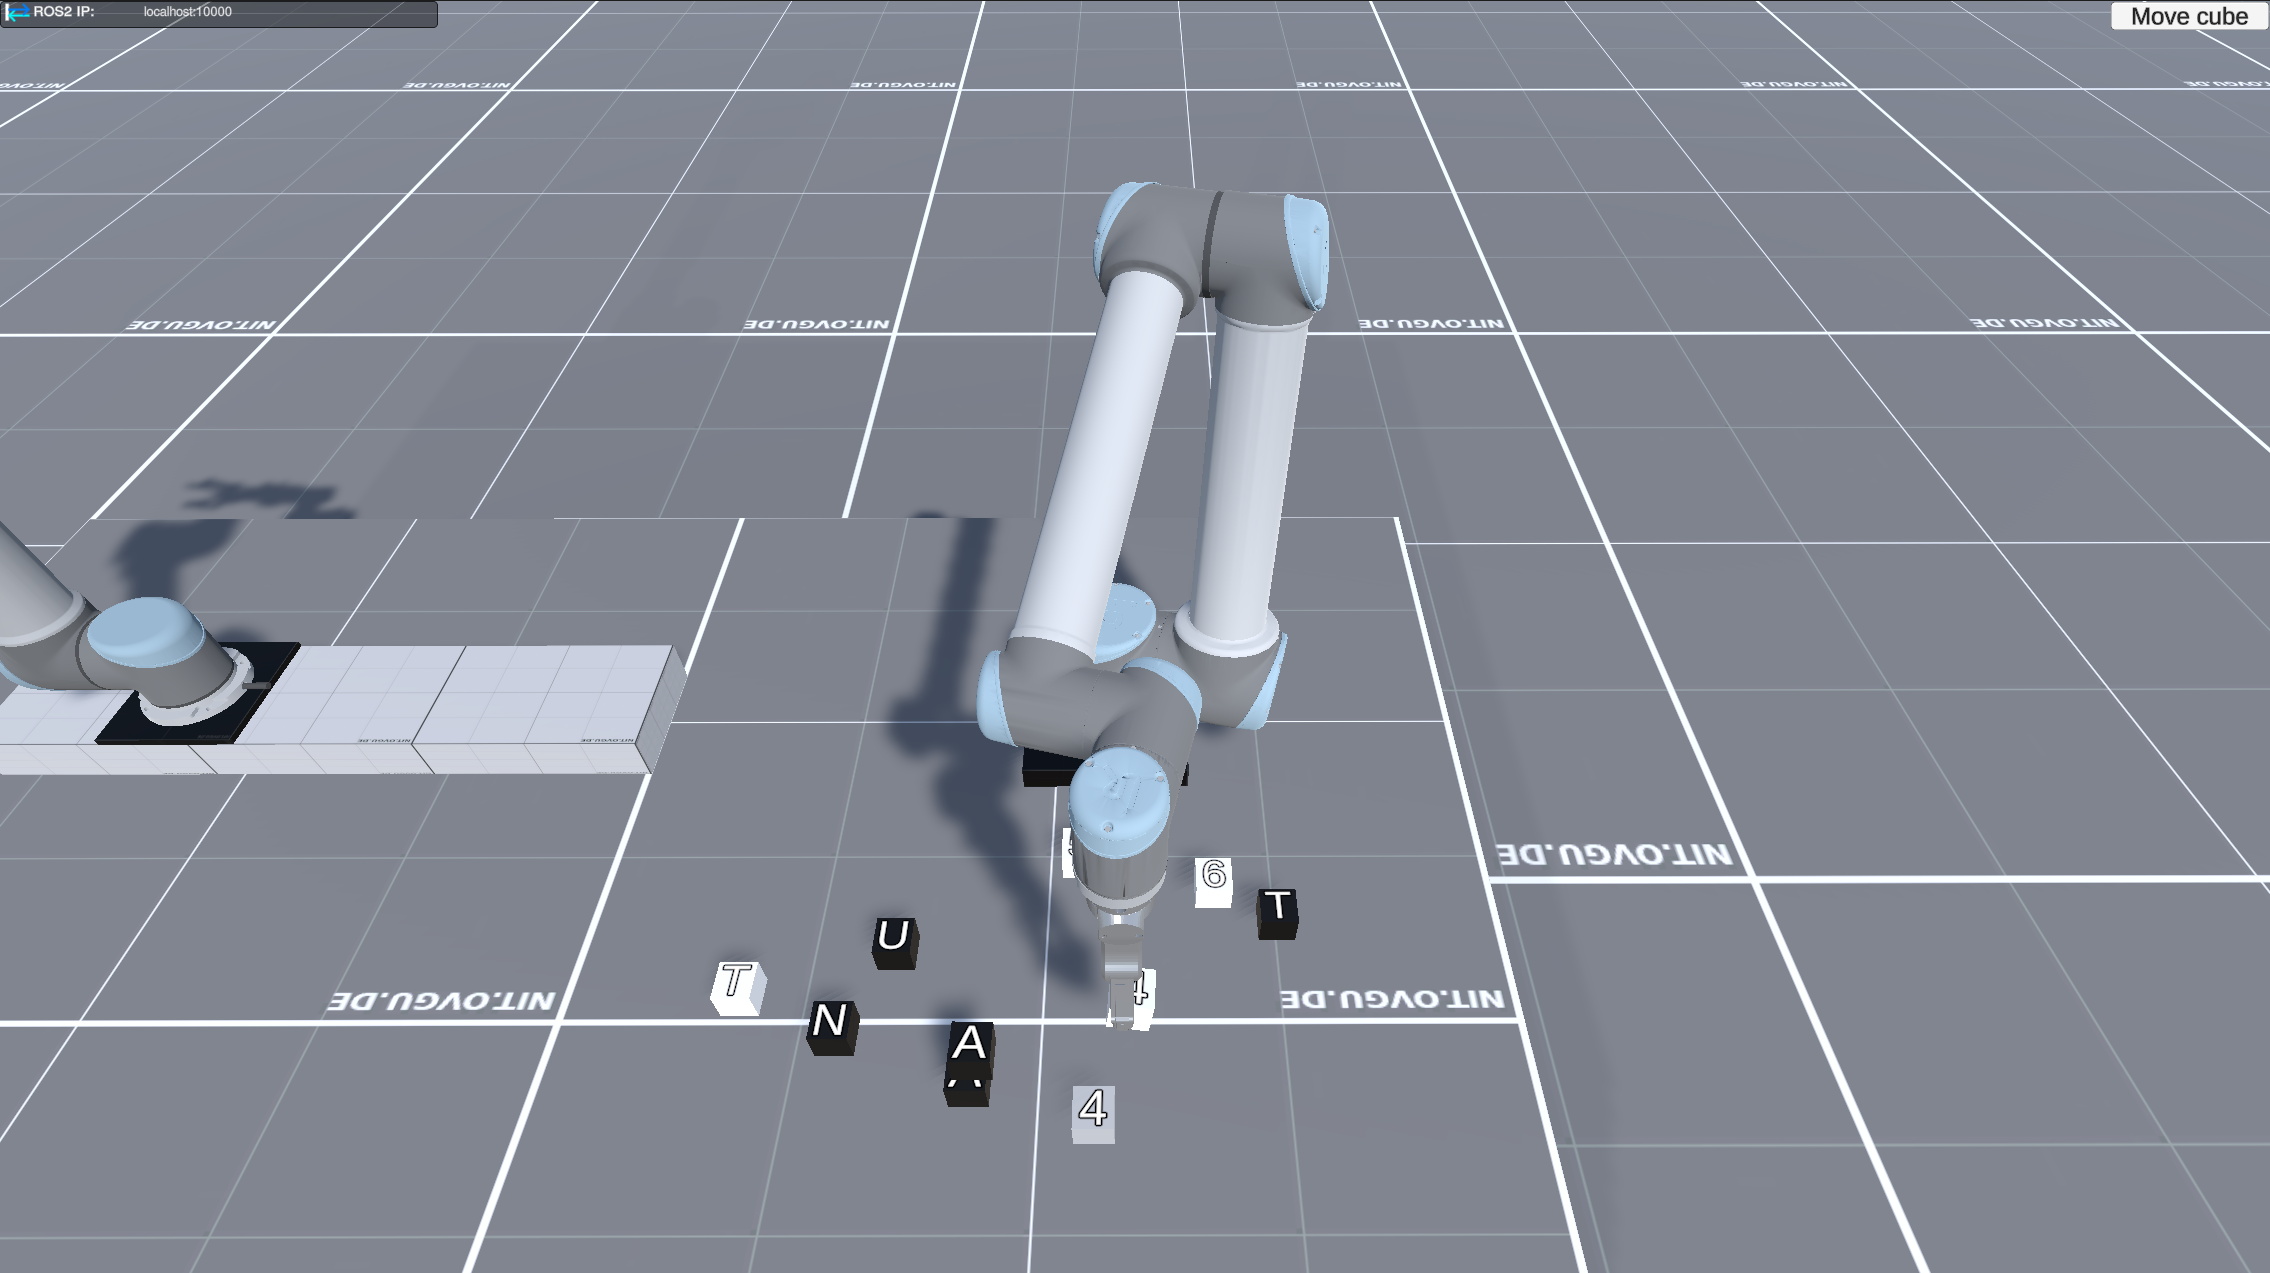
\includegraphics[width=0.3\linewidth]{media/Workspace 1_018.png}
    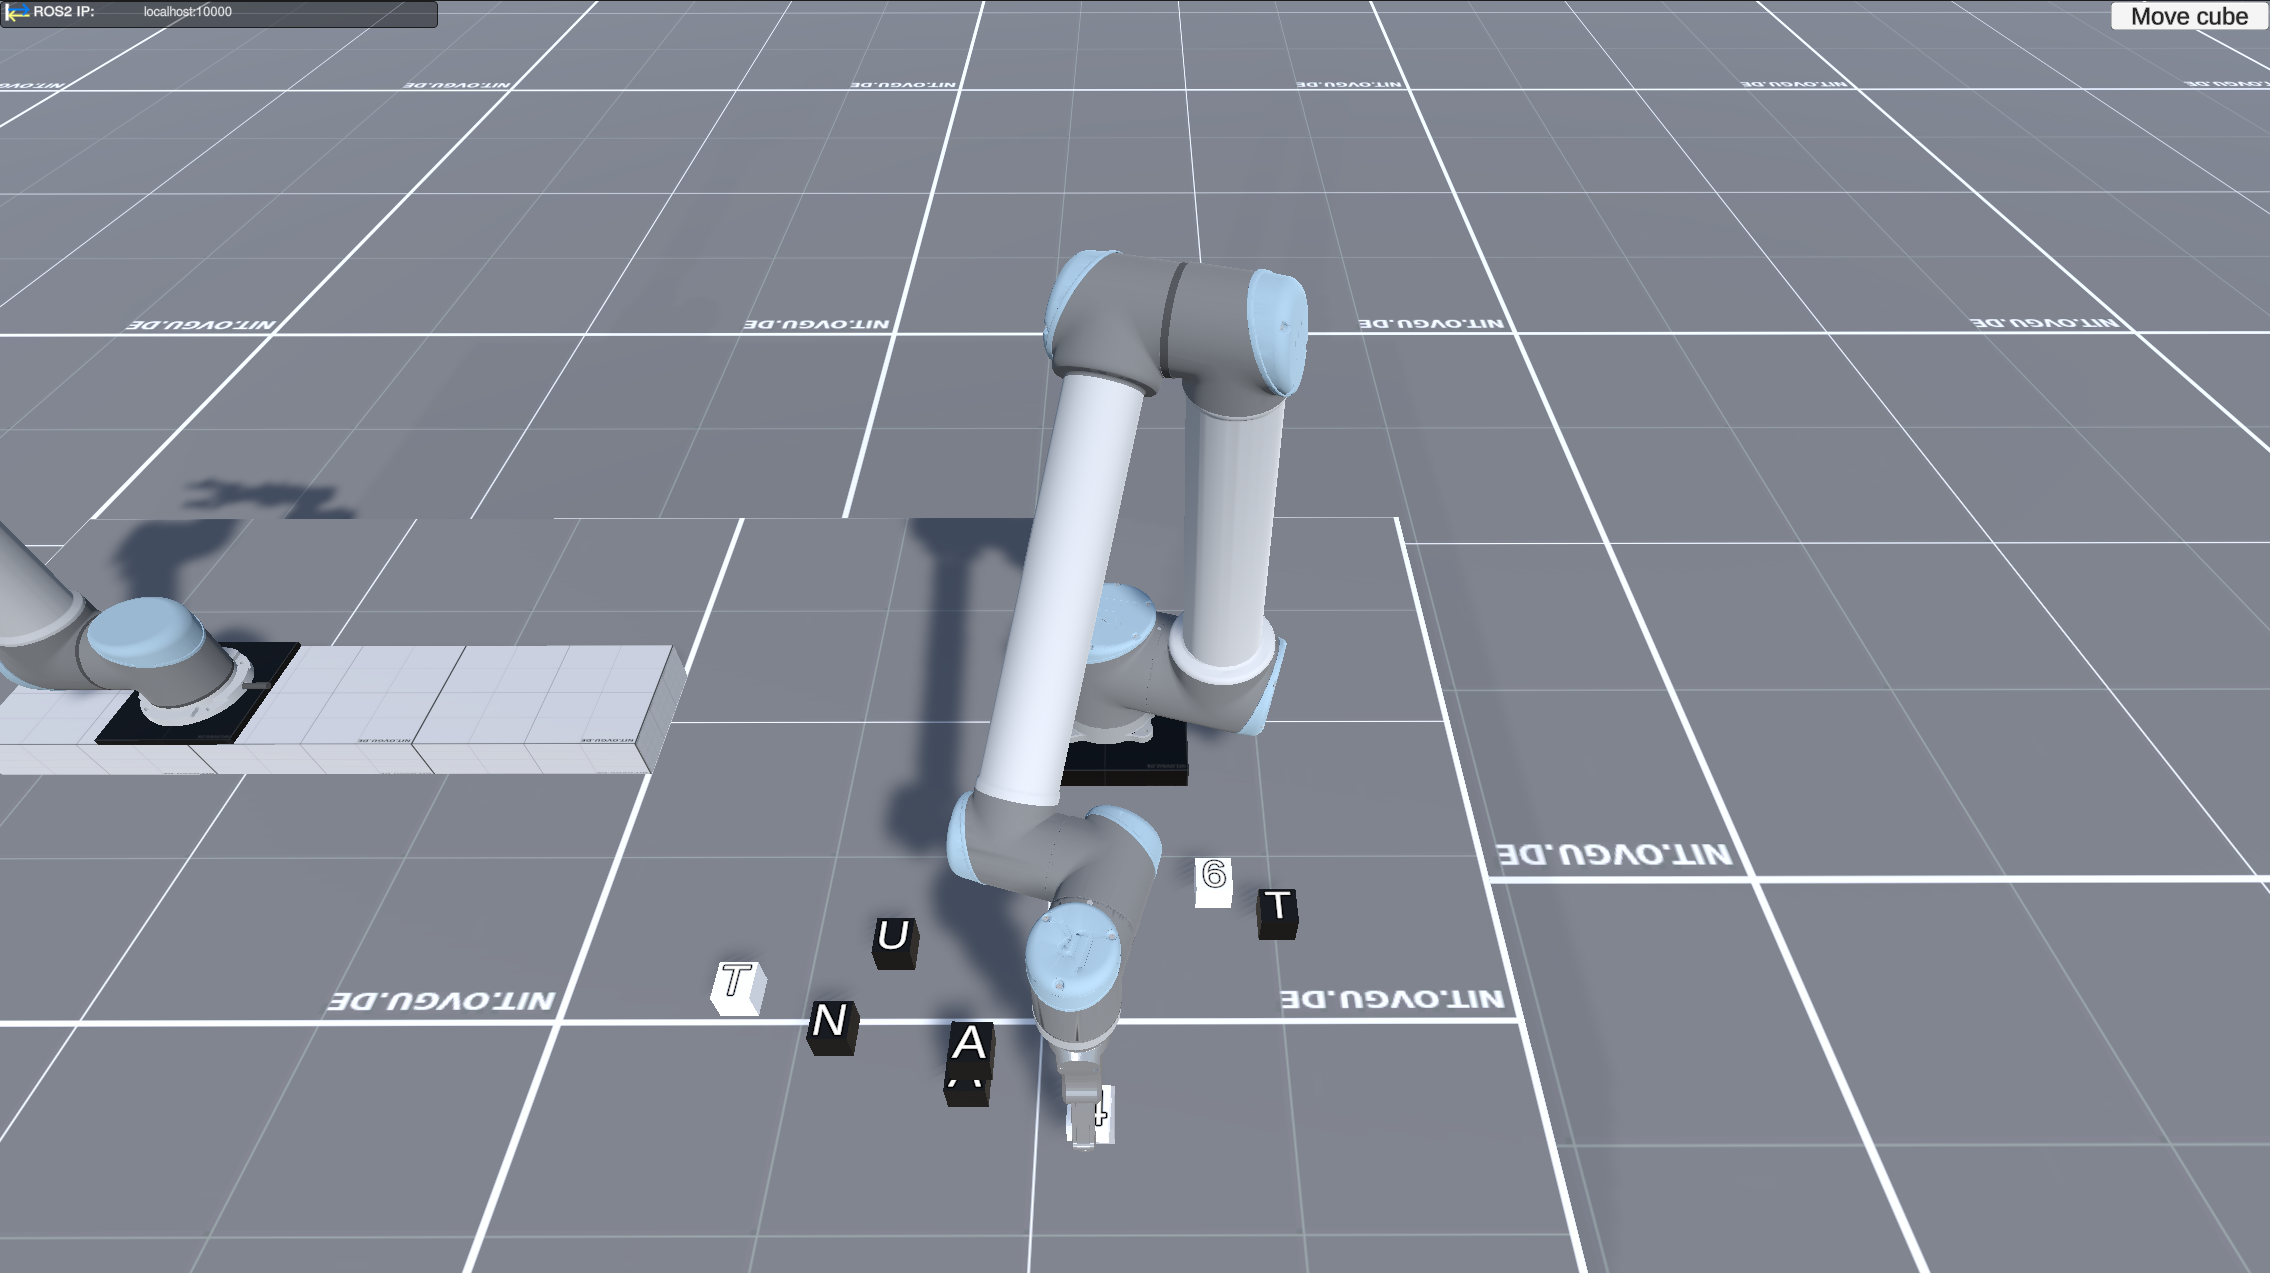
\includegraphics[width=0.3\linewidth]{media/Workspace 1_019.png}
    \caption{Manipulation eines erzeugten Würfels zu vorgegebener Zielposition in der Simulation.}
    \label{fig:cubemovement}
\end{figure}

\section{Conclusion}
\label{sec:conclusion}
This paper presents a proof of concept for a digital twin that mirrors a real-world workspace, including its objects, and uses \textit{MoveIt} to direct trajectories to physical robots by changing the digital environment.

XX


\section{Future Work}
\label{sec:future}
For the time being, the placement of cubes is limited by the accuracy with which they are detected. Currently, only the position and top letter are detected. However, an enhancement of the detection nodes is currently in development which will also estimate the 3D pose of the cube. With this feature, cubes can be spawned in all orientations around the workspace, leading to more dynamic motion planning. As cube detection is based on a YOLO network, it can also detect objects in the COCO dataset. Using the detected bounding box, depth values and a corresponding label, it would be possible to create such objects in real time. For example, a remote control has a rectangular shape. By identifying the difference in depth values, inside and outside the bounding box, a cuboid or some other shape can be generated. A label indicating the type of object can be added on top. If digital representations of these objects are already available, they can be scaled to the size detected and displayed in the digital workspace.

The pose estimation AI node uses mmpose to predict human poses and output the skeletal posture (COCO 17-point keypoint names[XX]) of people standing in front of the camera. The distance of each point is also taken from the depth image. This enables the person's model to be displayed correctly in front of the robot. Combining this model with virtual reality functionality gives the impression of standing right in front of the real robot, since the digital version can react to the virtual human.

Furthermore, the digital twin will be integrated into the lab system to control the real robots and vice versa. All features and programs running on the robot's ecosystem run one-to-one with the digital replicas.

\bibliography{egbib}





% \newpage
% \subsection{Paper length}
% Papers must not exceed 14 pages (excluding references). References and any appendices are unlimited.
% {\bf Only}  the acknowledgement and bibliography should be {\em excluded} from the page count: Papers must not have altered margins and formatting from those laid down by this style guide.

% The bibliography should begin immediately after the paper text.  It may
% be of any length, within reason.  It must {\em not} include
% annotations, figures, or any other paraphernalia intended to subvert the
% paper length requirement.

% % \begin{figure}
% % \begin{tabular}{ccc}
% % \bmvaHangBox{\fbox{\parbox{2.7cm}{~\\[2.8mm]
% % \rule{0pt}{1ex}\hspace{2.24mm}\includegraphics[width=2.33cm]{images/eg1_largeprint.png}\\[-0.1pt]}}}&
% % \bmvaHangBox{\fbox{\includegraphics[width=2.8cm]{images/eg1_largeprint.png}}}&
% % \bmvaHangBox{\fbox{\includegraphics[width=5.6cm]{images/eg1_2up.png}}}\\
% % (a)&(b)&(c)
% % \end{tabular}
% % \caption{It is often a good idea for the first figure to attempt to
% % encapsulate the article, complementing the abstract.  This figure illustrates
% % the various print and on-screen layouts for which this paper format has
% % been optimised: (a) traditional BMVC print format; (b) on-screen
% % single-column format, or large-print paper; (c) full-screen two column, or
% % 2-up printing. }
% % \label{fig:teaser}
% % \end{figure}

% \subsection{Citations}
% When citing a multi-author paper, you may save space by using ``{\em et
% alia}'', shortened to ``\etal'' (not ``{\em et.\ al.}'' as ``{\em et}'' is
% a complete word.)  The provided \verb'\etal' macro is a useful {\em aide
% memoire} in this regard.  However, use it only when there are three or more
% authors.  Thus, the following is correct: `` Frobnication has been trendy
% lately.  It was introduced by Alpher~\cite{Alpher02}, and subsequently
% developed by Alpher and Fotheringham-Smythe~\cite{Alpher03}, and Alpher
% \etal~\cite{Alpher04}.''

% This is incorrect: ``... subsequently developed by Alpher \etal~\cite{Alpher03} ...''
% because reference~\cite{Alpher03} has just two authors.  If you use the
% \verb'\etal' macro, then you need not worry about double periods
% when used at the end of a sentence as in Alpher \etal.

% %For this citation style, keep multiple citations in numerical (not
% %chronological) order, so prefer
% We use {\tt natbib}, so citations in random order are nicely sorted:
%  \cite{Alpher03,Alpher02,Authors06b,Authors06}.  However, we don't use the
% compress option, as we want each reference to have its own hyperlink and
% popup window.

% %-------------------------------------------------------------------------
% \subsection{Footnotes}

% Please use footnotes\footnote {This is what a footnote looks like.  It
% often distracts the reader from the main flow of the argument.} sparingly.
% Indeed, try to avoid footnotes altogether and include necessary peripheral
% observations in
% the text (within parentheses, if you prefer, as in this sentence).  If you
% wish to use a footnote, place it at the bottom of the column on the page on
% which it is referenced. Use Times 8-point type, single-spaced.


% \begin{figure*}
% \begin{center}
% \fbox{\rule{0pt}{2in} \rule{.9\linewidth}{0pt}}
% \end{center}
%    \caption{Example of a short caption, which should be centered.}
% \label{fig:short}
% \end{figure*}

% \begin{table}
% \begin{center}
% \begin{tabular}{|l|c|}
% \hline
% Method & Frobnability \\
% \hline\hline
% Theirs & Frumpy \\
% Yours & Frobbly \\
% Ours & Makes one's heart Frob\\
% \hline
% \end{tabular}
% \end{center}
% \caption{Results.   Ours is better.}
% \end{table}

% \subsection{Mathematics}

% Please number all of your sections and displayed equations.  It is
% important for readers to be able to refer to any particular equation.  Just
% because you didn't refer to it in the text doesn't mean some future reader
% might not need to refer to it.  It is cumbersome to have to use
% circumlocutions like ``the equation second from the top of page 3 column
% 1''.  (Note that the ruler will not be present in the final copy, so is not
% an alternative to equation numbers).  All authors will benefit from reading
% Mermin's description~\cite{Mermin89} of how to write mathematics.


% %-------------------------------------------------------------------------
% \subsection{References}

% List and number all bibliographical references in 9-point Times,
% single-spaced, at the end of your paper. When referenced in the text,
% enclose the citation number in square brackets, for
% example~\cite{Authors06}.  Where appropriate, include the name(s) of
% editors of referenced books.


% %------------------------------------------------------------------------
% \subsection{Color}

% Color is valuable, and will be visible to readers of the electronic copy.
% However ensure that, when printed on a monochrome printer, no important
% information is lost by the conversion to grayscale.


\end{document}
